\documentclass[12pt,letterpaper]{article}
\usepackage{pdfpages}
\usepackage{fancyhdr}
\usepackage[colorlinks=true, urlcolor=blue, linkcolor=blue]{hyperref}
\usepackage{graphicx}
\usepackage[top=1.4in, left=0.5in, right=0.5in, bottom=0.8in]{geometry}
\usepackage[T1]{fontenc}
\usepackage{helvet}
\pagestyle{fancy}
\renewcommand{\headrulewidth}{0pt}
\renewcommand{\footrulewidth}{0pt}
\setlength{\parindent}{0em}
\setlength{\parskip}{1em}


\fancyfoot[C]{\setlength{\unitlength}{1in}\begin{picture}(5,0)\put(-1.8,-1){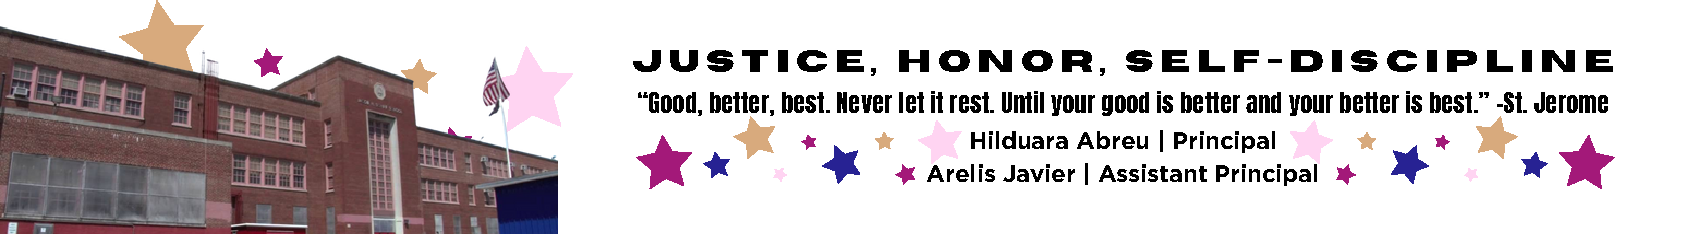
\includegraphics[width=8.8in,height=1.3in]{logo-1}}\end{picture}}
\fancyhead[C]{\setlength{\unitlength}{1in}\begin{picture}(5,0)\put(-1.9,-1){
\includegraphics[width=8.9in,height=1.3in]{logo-2}}\end{picture}}

\pagenumbering{gobble}
\addtolength{\evensidemargin}{-2in}
\addtolength{\topmargin}{-0.5in}
\addtolength{\textwidth}{0in}
%%%%%%%%%%%%%%%%%%%%%%%%%%%%%%%%%%%%%%%%%%%%%%%%%%%%%%%%%%%%%%%%%%

\begin{document}
\vspace*{0.5in}
Date: \href{https://www.ps192.org/apps/bbmessages/show_bbm.jsp?REC_ID=139439}{September 14, 2023} 

\textbf{Subject: Carta de Bienvenida Al Nuevo Año Escolar 2023-24}

Estimadas familias de 3-K y Pre-K,

¡Estamos emocionados contando los días hasta la llegada de nuestros estudiantes el jueves
7 de septiembre de 2023! Nuestros dedicados instructores y personal escolar esperan
ansiosamente darles la bienvenida a lo que promete ser un emocionante año de fomentar
conexiones y construir una sólida comunidad. Nuestros atentos educadores están emocionados
por compartir su alegría, energía y pasión por el aprendizaje con sus hijos.

Mientras nos preparamos para el regreso de su hijo, queremos compartir información 
importante que está en vigor en la PS 192 para garantizar una experiencia de aprendizaje
segura y placentera para todos. Por favor, tomen nota de las siguientes pautas:
	\begin{itemize}
	\item Uniformes: Todos los estudiantes deben venir vestidos con su uniforme escolar
	todos los días, que sigue siendo el mismo: una camisa burdeos y pantalones o faldas
	azul marino.
	\item Llegada y salida: Para garantizar un proceso de llegada y salida seguro y
	eficiente, tomen nota del siguiente horario. Habrá miembros del personal y señales que
	guiarán a las familias durante la primera semana de clases.  
		\begin{itemize}
		\item Llegada: Patio trasero a las 8:00 AM
		\item Salida: Patio trasero a las 2:15 PM
		\end{itemize}
	\end{itemize}
		
Primeros días de clases: Si bien todos los estudiantes tendrán un día escolar de 8:00 a 2:20 PM todos los días, los padres están invitados a quedarse con sus hijos el jueves y el
viernes de 8:00 a 10:00 AM para ayudar a nuestros jóvenes estudiantes a adaptarse de 
manera más fluida al entorno escolar.

Suministros escolares: PS 192 proporcionará todos los suministros escolares básicos, como
cuadernos, carpetas y crayones. Solo pedimos a las familias de 3K y PreK que proporcionen
una mochila, ropa de cambio y suministros para su siesta diaria (manta, sábana y/o un
pequeño objeto de transición como una muñeca o un peluche).

Nos sentimos privilegiados de ser parte de una comunidad donde padres, maestros, personal
y estudiantes trabajan juntos para construir relaciones sólidas que respalden el
crecimiento académico y social. Esperamos con ansias su participación en los diversos
eventos a lo largo del año escolar y les damos la bienvenida a su participación activa en
el viaje educativo de su hijo.
\pagebreak
\vspace*{1.5cm}
Las actualizaciones regulares sobre eventos en toda la escuela se comunicarán a través de
nuestro sitio web: \url{www.ps192.org}, \href{https://www.classdojo.com/}{ClassDojo}, School Messenger y nuestro grupo de WhatsApp. Si tienen alguna pregunta, no duden en ponerse en contacto con nuestra Coordinadora de Padres, Angela Rijo, en
\url{arijo@schools.nyc.gov}, sitio web de la escuela: \url{www.ps192.org/angela}, o al (646) 745-0150.

Realizaremos eventos a lo largo del año y esperamos colaborar con ustedes tanto en persona como virtualmente. Manténganse atentos para obtener más información sobre todos nuestros próximos eventos:
	\begin{itemize}
	\item El 14 de septiembre, organizaremos nuestro primer Encuentro Virtual con el
	Maestro de su hijo de 4:30 a 7:30 $($\href{https://www.ps192.org/apps/pages/index.jsp?uREC_ID=1504975&type=d&pREC_ID=2510452&tota11y=true}{Meet and Greet}$)$
	\item El 28 de septiembre, organizaremos nuestro primer Café con la Directora en
	persona a las 8:00 AM.
	\end{itemize}
 
Estamos emocionados de comenzar este año escolar y de interactuar con ustedes para
garantizar que su hijo disfrute de la mejor experiencia de aprendizaje posible, una en la
que se sientan valorados, alentados y emocionados por aprender y sus infinitas 
posibilidades.

Es un honor profundo servir como directora de la PS 192. Gracias por su inquebrantable
cooperación y dedicación a nuestros estudiantes, profesores y personal. Espero con ansias
colaborar con ustedes en el viaje educativo de su hijo.

En unidad,


\includegraphics[width=0.2\textwidth]{hil_signature}

\textbf{Principal}

\textit{La Escuela donde El Aprendisaje es Divertido!}

\url{www.ps192.org}

\end{document}
